\usetikzlibrary{arrows.meta,calc}
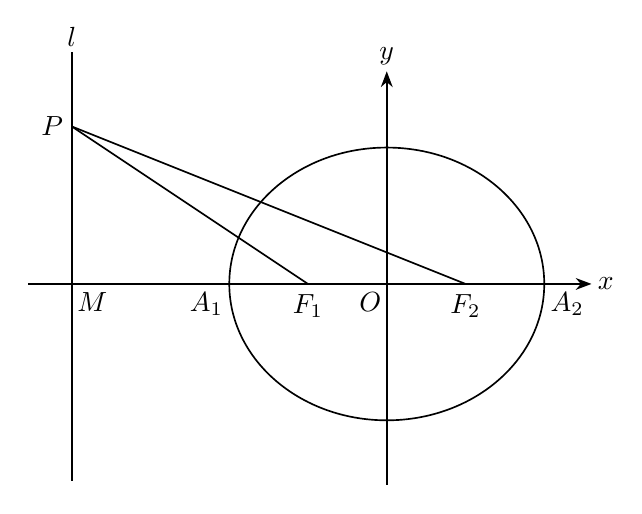
\begin{tikzpicture}[x=1cm,y=1cm,line width=.6pt,>=Stealth,font=\normalsize]
\coordinate (O) at (0,0);
\coordinate (M) at (-4,0);
\coordinate (A1) at (-2,0);
\coordinate (F1) at (-1,0);
\coordinate (F2) at (1,0);
\coordinate (A2) at (2,0);
\coordinate (P) at (-4,2);
\draw[->] (-4.55,0)--(2.6,0);
\draw[->] (0,-2.55)--(0,2.7);
\draw (O) ellipse [x radius=2, y radius=1.7320508];
\draw (-4,-2.5)--(-4,2.95);
\draw (P)--(F1);
\draw (P)--(F2);
\node[anchor=north east,inner sep=0pt] at (-0.06,-0.1) {$O$};
\node[anchor=north west,inner sep=0pt] at (-3.94,-0.1) {$M$};
\node[anchor=north east,inner sep=0pt] at (-2.07,-0.1) {$A_1$};
\node[anchor=north,inner sep=0pt] at (-1,-0.12) {$F_1$};
\node[anchor=north,inner sep=0pt] at (1,-0.12) {$F_2$};
\node[anchor=north west,inner sep=0pt] at (2.07,-0.1) {$A_2$};
\node[anchor=east,inner sep=0pt] at (-4.1,2) {$P$};
\node[anchor=south,inner sep=0pt] at (-4,3) {$l$};
\node[anchor=west,inner sep=0pt] at (2.67,0) {$x$};
\node[anchor=south,inner sep=0pt] at (0,2.77) {$y$};
\end{tikzpicture}
